\chapter{Methodology} \label{chap_3}
\ \\
The aim of this thesis was to analyze common automated testing campaigns, specifically OSS-Fuzz and FuzzBench as they are among the most popular ones, to see if there were any overlooked bugs in the projects that were integrated. This, in turn, meant studying their workflow and examining how programs are tested to verify how efficiently such frameworks are used by open-source developers.

What does it mean for a bug to be "overlooked" in this context?

If we think about OSS-Fuzz, where fuzzing is performed automatically by VMs, it means looking for cases where machines have failed: this could happen either due to a fault in the automation process or due to the integration choices made by the developers. In the former case, we may talk about limits imposed by OSS-Fuzz on its resources, like tests that cause out-of-memory scenarios, timeouts or even bugs that cannot be reliably and consistently reproduced (also called \textit{flaky)}. In the latter case, it is strictly related to the content of the \textit{project.yaml} configuration file: different sanitizers look for different types of bugs, while each fuzzing engine uses its own set of strategies to test a program, producing results that may be completely different from the other provided fuzzers. Given this, OSS-Fuzz was analyzed by taking a small selection of projects and testing them locally on the latest version with a fixed combination of fuzzing engine and sanitizers, using the latest public fuzzing queue available on the project's repository as the input corpus. 

If we think about FuzzBench, where projects are actively tested by several different fuzzers, it means to look for bugs discovered in older versions that were not tested on newer ones, which obviously is a human error. A small selection of projects from OSS-Fuzz are tested continuously by several different fuzzers, producing daily reports available both to the fuzzers and the chosen projects developers, along with public access to the corpora used to perform the tests as well as the results and the crashes found (if any). It is then responsibility of the project developers to analyze and fix these bugs, although this does not always happen. Given this, FuzzBench was analyzed by testing all available benchmarks and the ones from the SBFT '23 conference (see \ref{conference}), building the projects to their latest version with the same combination of fuzzing engine and sanitizers as OSS-Fuzz, and using as input corpus all the available crashes for each benchmark found in all fuzzing session that are publicly accessible between 2020 and October 2024 (at the moment of testing).

As previously mentioned, all relevant bugs were then appropriately reported to their respective developers.



\newpage
\section{Setting up the environment}
All tests were performed on two separate machines with similar specs, both equipped with personal installations of Ubuntu 22.04 LTS already run-in and used, using the following tools:
\begin{itemize}
    \item \textit{Docker} \cite{Docker}: virtualization tool used to run the different containers needed by OSS-Fuzz to create the environments where each projects was built and tested
    \item \textit{Valgrind} \cite{Valgrind_1}\cite{Valgrind_2}: dynamic binary instrumentation (DBI) framework with tools that perform analysis, profiling and management of a program during its execution, used specifically for the "Memcheck" tool when looking for memory-related bugs in fuzz targets built without sanitizers
    \item \textit{Python} (v. 3.10.12) \cite{python}: needed by OSS-Fuzz to provide its functionalities and used to create several scripts to perform information and web scraping, reports analysis and bug deduplication
    \item \textit{gsutil} \cite{gsutil}: command-line tool suite provided by Google to remotely access data stored on Google Cloud Service from your local machine, used to analyze FuzzBench experiments and download other resources
    \item \textit{Google Chrome/Development Driver} \cite{driver}: used during the information scraping phase of this work, discussed in section \ref{selection}
\end{itemize}

Regarding \textit{OSS-Fuzz}, most of the preparation was done using its GitHub repository, which was cloned locally on both machines. To provide its services, OSS-Fuzz uses several Python scripts that can be invoked from the command line with appropriate arguments: these commands can be used to update the repository and the files used to build each project, update the base images and each project image, build the project image and its fuzzers, and finally download other resources such as reports and publicly available corpora. 

Regarding \textit{FuzzBench}, most of the preparation was done by incorporating the \textit{gsutil} suite in a Python script that performed web scraping and downloaded content from its Google Cloud bucket, specifically on the section where all experiments results are collected.
\ \\

All tests were run by providing Docker with unlimited access to the CPU cores and disk space, while RAM was limited to 16GB, to ensure that no input may cause an out-of-memory situation that could result in a complete crash of the testing machine. 


\newpage
\section{OSS-Fuzz}
\subsection{Selecting the projects} \label{selection}
At the time of writing, the OSS-Fuzz campaign includes over 1000 projects that are actively being fuzzed and tested, but it would obviously be impossible to rebuild and test all of them locally due to the language heterogeneity of such projects and the knowledge and skills required to fix build errors. For this reason, this work focused exclusively on projects written in C/C++, as these languages are widely known to be prone to human error. Then, to further narrow down the analysis, I identified 5 different categories based on the number of sanitizers selected by the developers for testing, keeping ASan as the reference due to its popularity and efficiency. Finally, I ordered each set by "highest number of bugs issued" using the OSS-Fuzz bug tracker, and tested these lists from top to bottom until I had 5 projects for each category that were building and fuzzing correctly.

\begin{figure}[h]
\centering
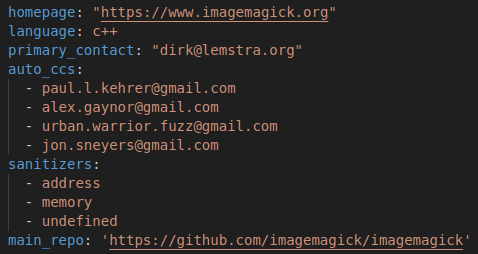
\includegraphics[scale=0.5]{foto/project_yaml.png}
\caption{Example of content from a project.yaml}
\label{fig:project_yaml}
\end{figure}

The first step in this process was to extract the list of all projects written in C/C++ and divide them according to the sanitizers used, and this was done by performing a preliminary analysis of the \textit{project.yaml} configuration file present inside each project's directory. To retrieve this information, I wrote a simple Python script taking as input the OSS-Fuzz "project" directory, iteratively explored each project's directory looking for the aforementioned configuration file, opened the file (assuming it was found) and scanned each line looking for the "language: c" string and the keywords "address", "memory" and "undefined", eventually saving the name of each project in the appropriate list.
\newline \newline
This yielded a total of 524 projects out of 1277 written using C/C++, with: 
\begin{itemize}
    \item 238 projects using all sanitizers when fuzzing
    \item 22 projects using ASan+MSan when fuzzing
    \item 62 projects using ASan+UBSan when fuzzing
    \item 46 projects using only ASan when fuzzing
    \item 156 projects not using any sanitizer when fuzzing
\end{itemize}

The next step was to determine the number of bugs already found for each project, and this required a thorough analysis of the OSS-Fuzz Issue Tracker website \cite{ossfuzz_bugtracker}. At the time of writing, the issue tracker platform has changed from "Monorail" to "Google Sites", so most of the work described here may no longer work as intended.

\begin{figure}[h]
\makebox[\textwidth][c]{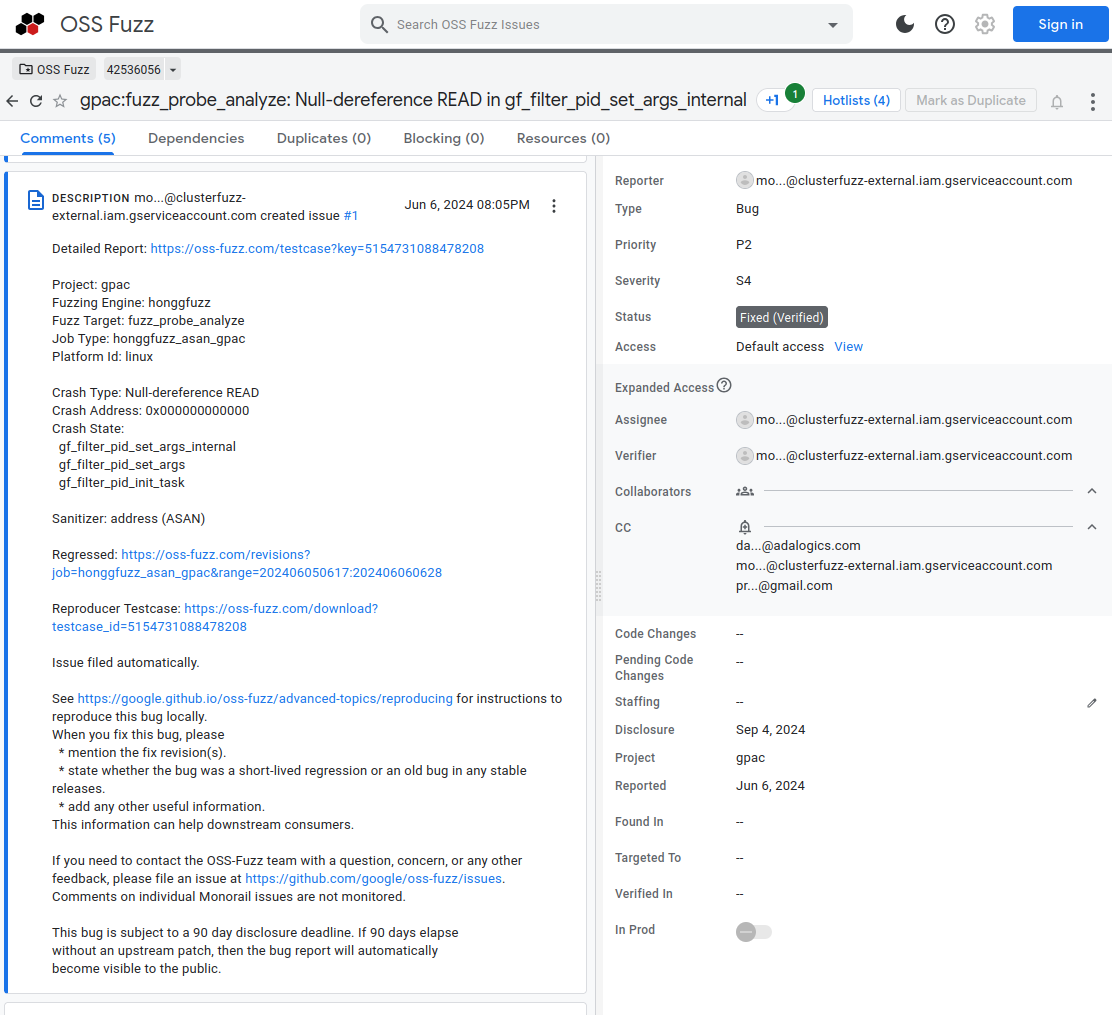
\includegraphics[width=0.65\paperwidth]{foto/issue.png}}
\caption{Example of bug report \cite{ossfuzz_bugtracker}}
\label{fig:issue}
\end{figure}

Since the Monorail APIs could only be accessed by the developers of projects already integrated into OSS-Fuzz, and there were no files that could be used for offline analysis, I had to perform web scraping on the individual issues from their web reports. To do this, I used as reference a GitHub repository written by Zhen Yu Ding called "Monorail Scraper" \cite{scraper}, a tool for scraping and retrieving data from Monorail-based platforms, which also included functionalities for ClusterFuzz-generated OSS-Fuzz issues. The tool relies on Google Chrome and its test development tool called "ChromeDriver" \cite{driver}, an autonomous web server implementing the "W3C WebDriver" \cite{driver_standard}, which in turn provides a remote interface to control user-agents and a set of interfaces to perform analysis and manipulation of DOM elements. Essentially, all these components combined allow the user to write scripts that, in turn, instruct the Google Chrome browser to visit a particular web page, analyze its DOM elements and possibly perform some interaction with it.


\newpage
The Python web-scraping script written requests a range of "report IDs" to be retrieved, then opens a new Google Chrome instance and performs a connection to a specifically constructed link on the Monorail website, attempting to reconnect only once if the first fails. If the resulting DOM displays a login form, it means that the requested bug is still in the disclosure window, in which case the next ID is analyzed. Assuming that the requested report is publicly available, the DOM is scanned for key information, finally stored in JSON files. 
\newline

This analysis was performed on all bugs between 2023-01-01 and 2024-06-31, for a total of 11743 collected reports.

\begin{figure}[h]
\makebox[\textwidth][c]{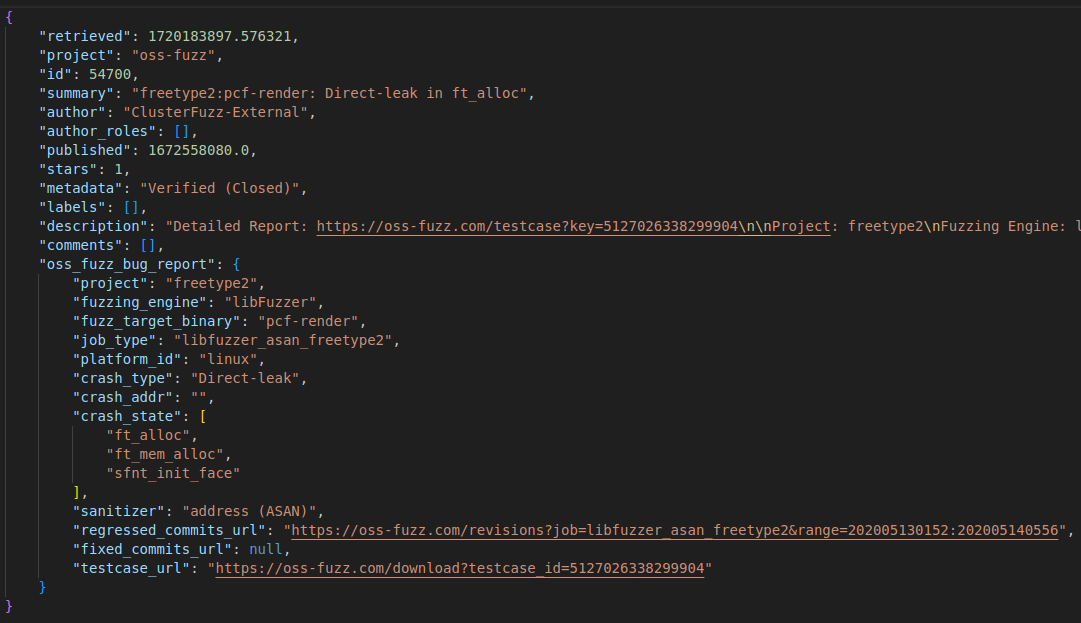
\includegraphics[width=0.7\paperwidth]{foto/json.png}}
\caption{Example of information collected from a report}
\label{fig:report}
\end{figure}


The second to last step was to analyze the JSON files and make a list of the most buggy projects for each category, which was done by writing a simple Python script that takes as input these files and analyzes the information fields collected, shown in the above figure. First, it checks the \textit{"metadata"} field for values such as "WontFix", "Duplicate" or "Invalid": the first means that the developers themselves tagged that specific bug as non-relevant and therefore will not be addressed in the future, the second refers to a report for a bug that has been already issued but was triggered by a different testcase, while the last one means that the reported bug could not be reliably reproduced using the provided testcase. Then, it checks the \textit{"description"} field for manual reports, that have been ignored as the information they contained were not always written according to the same standard used by ClusterFuzz and therefore not useful towards the collection of the information required. Assuming the report analyzed is valid and generated by ClusterFuzz, it retrieved the project name from the \textit{"oss\_fuzz\_bug\_report"} fields, using a dictionary key-value to keep track of the number of bugs reported for each project. 

\newpage
\begin{figure}[h]
\centering
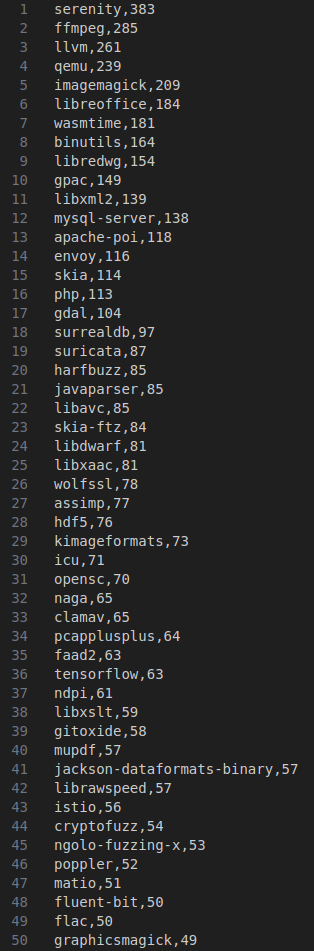
\includegraphics[scale=0.47]{foto/list.png}
\caption{Excerpt of the 50 most bugged projects}
\label{fig:list}
\end{figure}

The final step was to analyze all the bugs reported by each project individually and determine which fuzz target produced the highest number of reports. Given the previous script, I extended it to take the project name as input, so that the parsing of the JSON file focused only on reports for that particular project, and the dictionary key-value was now used to keep track of the number of bugs produced by each fuzzing target binary.


\newpage
All of this has resulted in the following projects and binaries being tested:
\begin{itemize}
  \item \textbf{All Sanitizers}
  \begin{itemize}
    \item binutils (fuzz\_objdump\_safe)
    \item harfbuzz (hb-subset-fuzzer)
    \item imagemagick (encoder\_heic\_fuzzer)
    \item libxml2 (valid)
    \item skia (skruntimeeffect)
  \end{itemize}
  \item \textbf{ASan + MSan}
  \begin{itemize}
    \item ghostscript (gs\_device\_pdfwrite\_fuzzer)
    \item libyang (lyd\_parse\_mem\_json)
    \item wasmedge (wasmedge-fuzztool)
    \item openjpeg (opj\_decompress\_fuzz\_J2K)
    \item myanmar-tools (zawgyi\_detector\_fuzz\_target)
  \end{itemize}
  \item \textbf{ASan + UBSan}
  \begin{itemize}
    \item cairo (svg-render-fuzzer)
    \item clamav (clamav\_dbload\_YARA\_fuzzer)
    \item freerdp (TestFuzzCoreClient)
    \item tarantool (luaL\_loadbuffer\_fuzzer)
    \item vlc (vlc-demux-dec-libfuzzer)
  \end{itemize}
  \item \textbf{ASan only}
  \begin{itemize}
    \item fwupd (uswid\_fuzzer)
    \item glslang (compile\_fuzzer)
    \item inchi (inchi\_input\_fuzzer)
    \item radare2 (ia\_fuzz)
    \item zeek (zeek-ftp-fuzzer)
  \end{itemize}
  \item \textbf{No Sanitizers}
  \begin{itemize}
    \item fluent-bit (flb-it-fuzz-cmetric\_decode\_fuzz\_OSSFUZZ)
    \item gpac (fuzz\_probe\_analyze)
    \item libdwarf (fuzz\_debug\_str)
    \item libredwg (llvmfuzz)
    \item serenity (FuzzJs)
  \end{itemize}
\end{itemize}





\subsection{Testing with OSS-Fuzz} \label{test}
The OSS-Fuzz repository contains several python scripts to build and test the available projects as well as debugging and reproducing crashes and bugs. Most of the tools used in this work are provided by the "helper.py" script, which I used to download a project's Docker image, build the fuzzers and download the lastest public corpora made available by the developers, using the following commands:
\begin{verbatim}
    $ python3 helper.py pull_images 

    $ python3 helper.py build_image {project_name}

    $ python3 helper.py build_fuzzers {project_name}
        --sanitizer={address(default),memory,undefined,none} 
            --engine={libfuzzer(default),afl, honggfuzz, centipede}
        
    $ python3 helper.py download_corpora 
        --project={project_name} --fuzz-target={binary_name}
\end{verbatim}

The \verb|pull_images| argument connects to OSS-Fuzz's Google Bucket to download and update all the Docker "base images" on your local machine, which are used by all projects as the base image to create their respective test environments.
The \verb|build_image| argument takes as input the name of a project and builds its Dockerfile, creating a new image on your local machine that will be later used to perform fuzzing. During this process, all dependencies and resources needed to correctly compile the fuzzers are downloaded and installed, including the main \textit{build.sh} script. It was used in conjunction with the previous command and daily \verb|git pull| on the OSS-Fuzz repository, to make sure that I was always building with the latest versions. 
The \verb|build_fuzzers| argument takes as input the name of a project, a list of possible sanitizers, a list of possible fuzzing engines to be used during the compilation of the fuzz targets. Although this command accepts only one sanitizer and fuzzing engine at a time, it's possible to mix them by acting on some environment variables provided by the base images. This command acts as a "wrapper" for a much more complex Docker command, that loads the project's Docker image using some specific environment variables and invokes the execution of the \textit{build.sh} script.
The \verb|download_corpora| argument takes as input a project name and a fuzz target, it then connects to the project's Google Bucket and downloads the latest public corpus for the provided fuzz target.

After executing these commands, three new directories are created: \verb|out| contained the project's directory where all built files were saved, including libraries, fuzz targets and other files created by the selected fuzzer, \verb|work| acted as a temporary location to store intermediate files during the building process and the fuzzing sessions, and \verb|corpus| contained the downloaded corpora stored as a zip file.

To prepare the tests, I was tasked with building the chosen fuzz targets using AFL++ (current state-of-the-art fuzzer) and with all possible sanitizers, meaning that each project was compiled 4 times: with ASan only, with MSan only, with UBSan only and without any sanitizer.

The tests were performed inside each project's Docker image, created and configured using the following command:

\begin{verbatim}
    $ docker run --rm --privileged 
        --platform linux/amd64 --memory=16g 
        -v /oss-fuzz/build/out/{project_name}/:/out/
        -v /oss-fuzz/build/corpus/{project_name}/:/corpus/    
        -v /home/zio-saba/Scrivania/TESI/logfiles/:/logfiles/ 
        -it  gcr.io/oss-fuzz/{project_name} /bin/bash
\end{verbatim}
The first parameters are needed to create a privileged instance of Docker, specify the running platform on which the fuzz targets will be tested and limit memory inside the container. The arguments starting with \verb|-v| are used to create a shared directory, i.e. linking a local directory to a virtual one created inside the container: this was necessary to make sure that I could access the resources stored locally on my machine (i.e. fuzz targets, libraries and their corpus) from inside the Docker container. The last line invokes the project image to load as well as making it interactive by spawning a \verb|/bin/bash| process.
\ \\

Once the Docker image has been loaded and ready to use, some final adjustments were performed to perform the tests, here we mention few of them:
\begin{itemize}
    \item all tests performed on fuzz targets built with MSan required the sanitizer's libraries to be copied in some specific locations, using the following commands:
\begin{verbatim}
$ cp -R /usr/msan/lib/* /usr/local/lib/x86_64-unknown-linux-gnu/
$ cp -R /usr/msan/include/* /usr/local/include
\end{verbatim}
    \item all tests performed on fuzz targets built without sanitizers relied on Valgrind to perform binary analysis and profiling, installed using the following command:
\begin{verbatim}
$ sudo apt install gdb valgrind
\end{verbatim}
    \item sometimes, the \verb|apt| tool was not available in a specific Docker container, because all base images provided by OSS-Fuzz contain a minimal installation with only some key packages that are usually enough to compile a programs, such as compiler, assembler, text editors and standard libraries: in such cases, the \verb|unminimize| command was executed, which essentially "unpacks" the container and reverts it to a standard Ubuntu image, reinstalling all the default packages as well as standard additional tools
\end{itemize}












\newpage
When testing fuzz targets built with ASan, MSan or UBSan, I used the following command:
\begin{verbatim}
    $ for i in /corpus/*; do 
        echo "TEST" $i; 
        echo "TEST" $i >> /logfiles/PROJECT_SANITIZER-NAME.log; 
        ./{fuzz_target} $i &>> /logfiles/PROJECT_SANITIZER-NAME.log; 
      done
\end{verbatim}
The shell \verb|for| construct scans all files found in the "corpus" directory, then prints the name of the current testcase on the terminal for monitoring purposes, and finally logs the name of the current testcase and the results of the fuzz target executed on that particular testcase on a log file.

\begin{figure}[h]
\makebox[\textwidth][c]{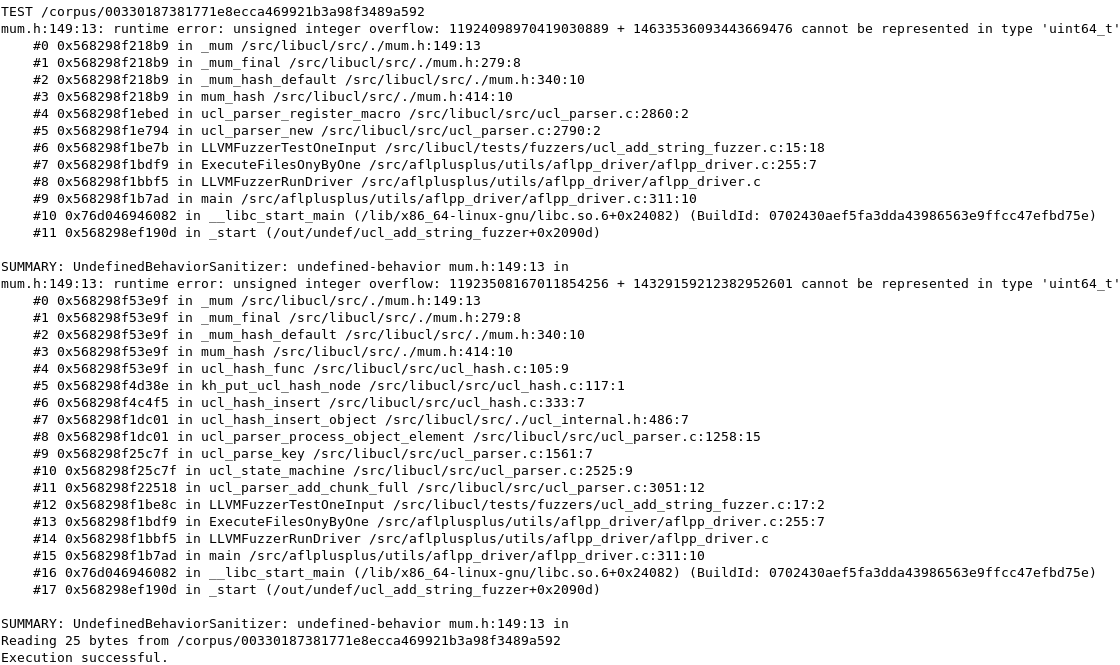
\includegraphics[width=0.8\paperwidth]{foto/ubsan_example.png}}
\caption{Example of integer-overflow bug reported by UBSan}
\label{fig:ubsan_example}
\end{figure}





\newpage
When testing fuzz targets built without any sanitizers, I used Valgrind to analyze and profile the binary's execution, using the following command:
\begin{verbatim}
    $ for i in /corpus/*; do 
        echo "TEST" $i; 
        valgrind --log-fd=9 9>>/logfiles/PROJECT_valgrind.log 
            ./{fuzz_target} $i >> /logfiles/PROJECT_valgrind.log 
            && echo -e "\n\n" >> /logfiles/PROJECT_valgrind.log; 
      done
\end{verbatim}
Similarly to before, the shell \verb|for| construct scans all files found in the "corpus" directory and prints the name of the current testcase on the terminal for monitoring purposes, then Valgrind is invoked with a custom file descriptor to redirect \verb|STDERR| in the log file, and the name of the current testcase and the results of the fuzz target executed on that particular testcase are logged on a log file.

\begin{figure}[h]
\makebox[\textwidth][c]{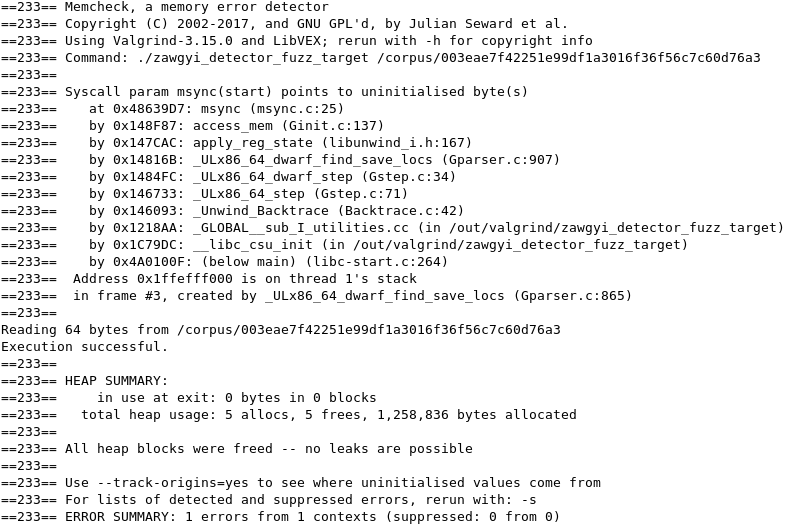
\includegraphics[width=0.65\paperwidth]{foto/valgrind_example.png}}
\caption{Example of use-of-uninitialized-memory (UUM) bug reported by Valgrind}
\label{fig:valgrind_example}
\end{figure}



\newpage
However, not all projects built on their first attempt.
In most cases, the building process failed due to missing libraries: for example, libraries like \verb|pthread| and \verb|math| were often automatically added by the sanitizers. Other times, libraries were not being correctly linked and/or were missing crucial compiling flags, like \verb|-ldl| and \verb|-lz|. To fix these problems, I had to manually modify the source files and compile the fuzz targets from inside the Docker container, using the following command:
\begin{verbatim}
    $ docker run --rm --privileged --platform linux/amd64 
        -e PROJECT_NAME={project_name} -e HELPER=True 
        -e FUZZING_LANGUAGE=c++ 
        -e FUZZING_ENGINE=afl 
        -e SANITIZER={address,memory,undefined,none} 
        -v /oss-fuzz/build/out/{project_name}/:/out/   
        -v /oss-fuzz/build/work/{project_name}/:/work/
        -it  gcr.io/oss-fuzz/{project_name} /bin/bash
\end{verbatim}
Similarly to before, the first parameters are needed to create a privileged instance of Docker and specify the running platform on which the fuzz targets will be tested, the arguments starting with \verb|-v| are used to create a shared directory in the Docker container and the last line invokes the project image to load as well as making it interactive by spawning a \verb|/bin/bash| process.
The novelty lies in the arguments starting with \verb|-e|, which can be used to override the environment variables provided by the Docker image: these variables can be used by the source files to compile a program using the most appropriate compile flags, fuzzing engine and sanitizers, and they can be easily modified by the user when creating the Docker image to easily re-target the compilation with little to none effort. 

After loading the Docker image and modifying the source files, the command \verb|compile| invokes the execution of the "build.sh" script and starts the building process for the fuzz targets.













\newpage
\section{FuzzBench}
\subsection{Selecting the projects}
As previously mentioned, the FuzzBench campaign started in 2020, performing tests almost daily for the past 4 years while providing valuable information to both fuzzers developers and the developers of the selected projects that have been integrated as benchmarks.
\begin{figure}[h]
\centering
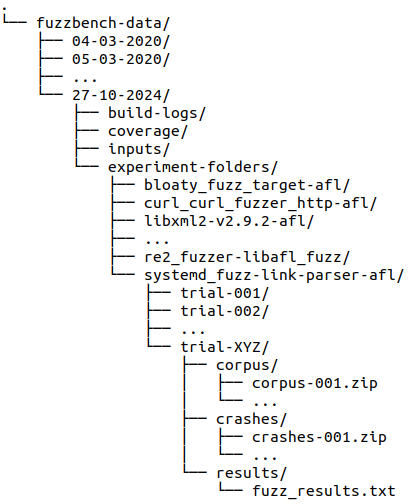
\includegraphics[scale=0.4]{foto/tree.png}
\caption{Simplified structure of the FuzzBench's Google Cloud directory tree}
\label{fig:tree}
\end{figure}
\ \\
All data on FuzzBench is grouped by test date, and each test set is composed by several key information:
\begin{itemize}
    \item \verb|build-logs|: contains the logs generated when building the fuzz targets
    \item \verb|coverage|: contains information related to the coverage achieved by each fuzzer on the different projects tested that day
    \item \verb|input|: contains the binaries executed to compile the different fuzz targets
    \item \verb|experiment-folders|: contains all the data related to the testing sessions
\end{itemize}

Following the experiments, each project has its own folder that specifies the name of the project, the fuzz target tested, the fuzzing engine used and sometimes also the objective of the session (bugs, coverage, correctness). Each project then undergoes several fuzzing sessions, identified by different \verb|trial| folders, providing all the information that were relevant to this work:
\begin{itemize}
    \item \verb|corpus|: contains several corpora stored as zip files.
    \item \verb|crashes|: contains all the crashes found in each trial as a separate zip file
    \item \verb|results|: contains the cumulative log of all fuzzing sessions
\end{itemize}


The objective of this analysis was to build the latest version of several experiments, download all the available \verb|crashes| for each one of them and verify whether they have been fixed or not. However, preliminary analysis yielded over 100 milion possible zip files to download and test, which would require several months of work by itself. 
As previously mentioned, FuzzBench provides coverage-oriented or bug-oriented fuzzing, therefore I focused on bug-oriented experiments for the analysis. To do this, I found the \textit{experiment-requests.yaml} configuration file \cite{exp_yaml} inside the FuzzBench repository, which contained all information related to the type of tests conducted, the projects tested as well as all the fuzzing engines used:

\begin{figure}[h]
\centering
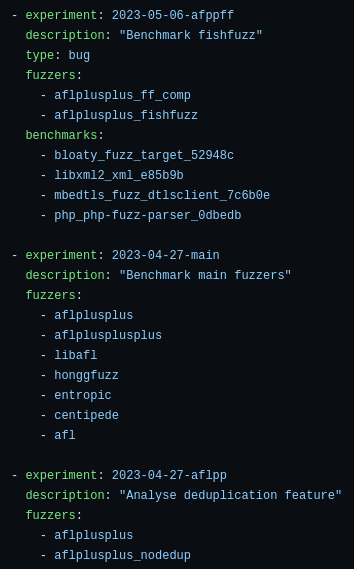
\includegraphics[scale=0.58]{foto/exp_yaml.png}
\caption{Excerpt from the experiment configuration file}
\label{fig:exp_yaml}
\end{figure}

Similarly to the process shown in section \ref{selection}, I wrote a simple Python script taking as input the above file and storing the name of all those experiments containing the string "type: bug". Unfortunately, this file only contained information on all experiments between 2020 and 2023, forcing me to later retrieve all the experiments performed in 2024.

Regarding the selection of the projects and fuzz targets to test, while the initial idea was to perform the analysis only on the benchmarks provided by FuzzBench, it was later decided to also include the special benchmarks added during the "SBFT '23" conference (refer to \ref{conference}) due to the overwhelmingly amount of bugs discovered when performing preliminary tests on them.

Finally, to retrieve all possible crashes from the bug-oriented experiments performed in 2020-2023 and all experiments from 2024, I used the \textit{gsutil} suite provided by Google, which works similarly to the \verb|ls|, \verb|mv| and \verb|cp| command of the Linux shell, except that it takes as argument the URL of a Google Cloud resource. To construct the URL of all the resources needed, I wrote a Python script that essentially performs horizontal scraping over the directory tree shown before (Figure \ref{fig:tree}), storing at each intermediate steps the link of the next resource to list using the \verb|gsutil ls| command.
\ \\ 

In conclusion, this analysis yielded 971656 zip file, a total of 9 milion crashes to test, and the following projects and fuzz targets being tested:

\noindent
\begin{tabularx}{\textwidth}{
    @{\hspace{2em}}% Space for left bullet
    >{\leavevmode\llap{\textbullet~}\raggedright\rule{0pt}{4ex}}% Left bullet + formatting of column
    X% Left column specification
    @{\quad\hspace{1em}}% Space between columns + right bullet space
    >{\leavevmode\llap{\textbullet~}\raggedright\arraybackslash}% Right bullet + formatting of column
    X% Right column specification
    @{}% No column space on right
  }
  arrow (parquet-arrow-fuzz) & aspell (aspell\_fuzzer) \\
  assimp (assimp\_fuzzer) & bloaty (fuzz\_target) \\
  curl (curl\_fuzzer\_http) & ffmpeg (ffmpeg\_demuxer\_fuzzer) \\
  file (magic\_fuzzer) & freetype2 (ftfuzzer) \\
  grok (grk\_decompress\_fuzzer) & harfbuzz (hb-shape-fuzzer) \\
  jsoncpp (jsoncpp\_fuzzer) & lcms (cms\_transform\_fuzzer) \\
  libaom (av1\_dec\_fuzzer) & libjpeg-turbo (libjpeg\_turbo\_fuzzer) \\
  libpcap (fuzz\_both) & libpng (libpng\_read\_fuzzer) \\
  libxml2 (xml) & mbedtls (fuzz\_dtlsclient) \\
  openssl (x509) & openthread (ot-ip6-send-fuzzer) \\
  php (php-fuzz-parser) & proj4 (proj\_crs\_to\_crs\_fuzzer) \\
  re2 (re2\_fuzzer) & sqlite3 (ossfuzz) \\
  systemd (fuzz-link-parser) & vorbis (decode\_fuzzer) \\
  woff2 (convert\_woff2ttf\_fuzzer) & zlib (zlib\_uncompress\_fuzzer)  
\end{tabularx}





\newpage
\subsection{Testing with FuzzBench}
FuzzBench projects were build and tested almost identically to the methodology shown for OSS-Fuzz (see \ref{test}), except for few small differences.

Initially, I used the "helper.py" script to download the latest Docker image for each project, but the fuzzers had to be built manually:
this is because all FuzzBench benchmarks are compiled using a custom combination of sanitize flags from ASan and UBSan \cite{flags}, implying that FuzzBench does not perform memory analysis when fuzzing. To replicate this build configuration I had to modify the environment variables provided by the Docker images, using with the following command:
\begin{verbatim}
    $ docker run --rm --privileged 
        --platform linux/amd64 --memory=16g 
        -e PROJECT_NAME={project_name} -e HELPER=True 
        -e FUZZING_LANGUAGE=c++ -e FUZZING_ENGINE=afl 
        -e SANITIZER=address 
        -e SANITIZER_FLAGS_address="
            -fsanitize=address,array-bounds,bool,builtin,enum,
                integer-divide-by-zero,null,object-size,return,
                returns-nonnull-attribute,shift,
                signed-integer-overflow,
                unsigned-integer-overflow,
                unreachable,vla-bound,vptr
            -fno-sanitize-recover=array-bounds,bool,builtin,enum,
                integer-divide-by-zero,null,object-size,return,
                returns-nonnull-attribute,shift,
                signed-integer-overflow,unreachable,
                vla-bound,vptr 
            -fsanitize-address-use-after-scope" 
        -v /oss-fuzz/build/out/{project_name}/:/out/  
        -v /oss-fuzz/build/work/{project_name}/:/work/
        -v /oss-fuzz/build/corpus/{project_name}/:/corpus/
        -v /home/zio-saba/Scrivania/TESI/logfiles/:/logfiles/  
        -it  gcr.io/oss-fuzz/{project_name} /bin/bash
\end{verbatim}
As previously shown, the first parameters are needed to create a privileged instance of Docker, specify the running platform on which the fuzz targets will be tested and limit the container memory usage, the arguments starting with \verb|-e| override the environment variables provided by the Docker image, the arguments starting with \verb|-v| are used to create shared directories and the last line invokes the project image to load as well as making it interactive by spawning a \verb|/bin/bash| process.
Given that the container accepts only one sanitizer at a time, I had to specify both ASan and UBSan flags in the same variable storing the ASan sanitizer flags, using as reference the subset of UBSan flags used by default by FuzzBench \cite{flags}.

\newpage
All crashes collected during the initial analysis were then categorized as follows:
\begin{itemize}
    \item \textbf{crash:} inputs leading to any scenario that forces the system to close the process, like SEGV and heap/stack buffer overflows
    \item \textbf{out-of-memory (oom):} inputs inducing memory leaks or using huge allocation sizes to purposely test fail-safe mechanisms
    \item \textbf{timeout:} inputs that are either very long to parse or that purposely introduce unnecessary operations, again to test the resiliency of the program 
\end{itemize}

Finally, tests were performed using the following command:
\begin{verbatim}
    $ for i in /corpus/*; do 
        echo "TEST" $i; 
        echo "TEST" $i >> /logfiles/PROJECT_SANITIZER-NAME.log; 
        timeout 30s ./{fuzz_target} $i 
            &>> /logfiles/PROJECT_SANITIZER-NAME.log; 
      done
\end{verbatim}
As before, the shell \verb|for| construct scans all files found in the "corpus" directory, then prints the name of the current testcase on the terminal for monitoring purposes, and finally logs the name of the current testcase and the results of the fuzz target executed on that particular testcase on a log file. The only addition is the \verb|timeout| command, and that is because due to the presence of inputs that purposely take unnecessary time, I decided to follow the same timeout duration used by ClusterFuzz when fuzzing with AFL++ \cite{timeout}.